\Needspace{6\baselineskip}
\subsection{Mounted Pilot Calibration}
Table~\ref{tab:rgb} and Figure~\ref{fig:rgb-results} summarize the raw calibration readings. The red condition has a dominant red response and substantially higher total light than the green condition. The green reference has a larger green than red component, despite much lower absolute counts. The clear channel therefore helps separate overall illumination from normalized color. The unlit condition produced small nonzero readings, making a dark threshold more appropriate than exact equality to zero.

\begin{table}[htbp]
\centering
\caption{Median raw counts transcribed from the mounted RGB calibration photographs, with 154~ms integration and 4$\times$ gain.}
\label{tab:rgb}
\begin{tabular}{lrrrr}
\toprule
Pilot condition & R & G & B & Clear \\
\midrule
Red &301&25&34&331\\
Green &17&22&8&46\\
Unlit &4&3&3&5\\
\bottomrule
\end{tabular}
\end{table}

\begin{figure}[htbp]
\centering
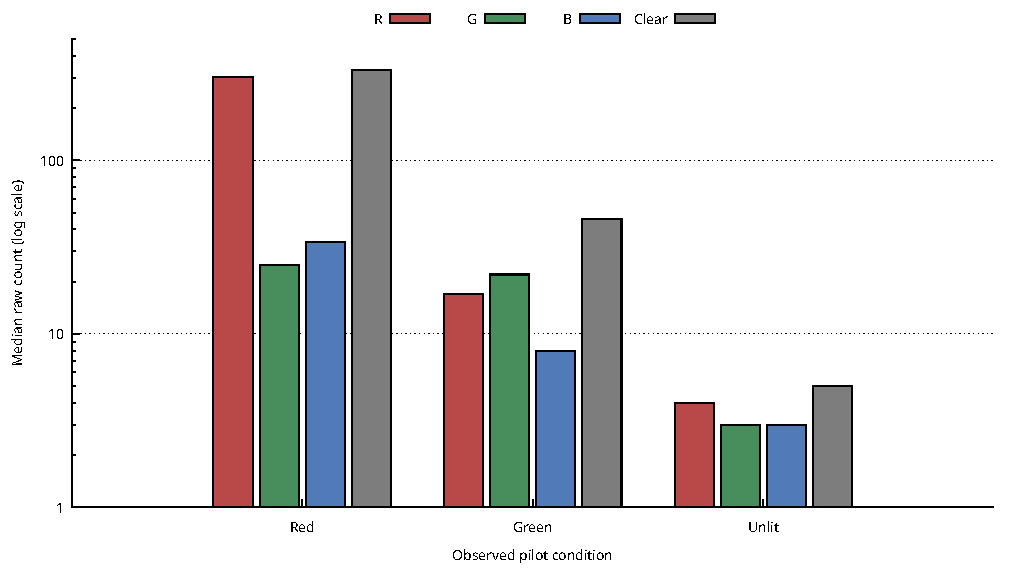
\includegraphics[width=0.88\linewidth]{figures/rgb_calibration.pdf}
\caption{Original result figure generated from the calibration readings in Table~\ref{tab:rgb}. The vertical axis is logarithmic. Each group contains the median red, green, blue, and broadband clear-channel response.}
\label{fig:rgb-results}
\end{figure}

The photographs contain overlapping readings, so the transcribed rows are not independent repetitions. These medians establish calibration references for the fixed, shielded alignment, rather than a measured classification accuracy across different lighting conditions. The selected 0.07 distance tolerance covers the recorded red and green samples; broader robustness requires testing the assembled optical geometry.

\Needspace{6\baselineskip}
\subsection{Mechanical and Software Checks}
The supervised power-button trial registered an on action with servo A configured to press at 29 degrees on the tape-mounted mechanism. Its configured rest position is 0 degrees. This is an angular setting for that mounting, not a measurement of contact force or repeated-actuation reliability. The photograph in Figure~\ref{fig:prototype} provides the corresponding appliance context.

Table~\ref{tab:control-checks} summarizes the software checks performed on the integrated implementation. The backend suite passed 20 tests, and the embedded adjustment checks exercised all 46$\times$46 pairs of allowed initial and target setpoints. Host checks used the actual heater-control header with stubbed peripherals, so these results verify command decisions separately from mechanical behavior.

\begin{table}[htbp]
\centering
\caption{Verified software behavior and its interpretation.}
\label{tab:control-checks}
\small
\begin{tabularx}{\linewidth}{@{}P{3.2cm}L@{}}
\toprule
Check & Observed result \\
\midrule
Unknown startup state & No automatic toggle is issued to discover power; unknown setpoint remains unsynchronized.\\
Standby command & Wake is separated from the requested action, which waits for a fresh pilot observation.\\
Missing confirmation & The pending action is cancelled without repeating wake presses indefinitely.\\
Circular setpoint & The 30-to-75 downward boundary and 75-to-30 upward boundary are one-step software transitions.\\
Temperature distinction & Captures taken during adjustment remain unavailable as measured water temperature until a later capture.\\
User cancellation & A later on request can cancel a pending off action during the wake sequence.\\
\bottomrule
\end{tabularx}
\end{table}

The controller firmware compiled successfully. Together with the optical and button observations, these checks support the separation of sensing, decision logic, and physical actuation. They do not quantify water-use accuracy or energy savings; the prototype reports panel observations and configured pulse-based quantities rather than independently calibrated tank temperature or electrical consumption.
